\section{Phân tích khám phá dữ liệu đa phương thức}

Quá trình phân tích khám phá dữ liệu đóng vai trò nền tảng trong việc thấu hiểu bản chất tập dữ liệu, từ đó định hướng thiết kế không gian đặc trưng. Dựa trên tính chất phi cấu trúc của bài toán, nội dung được quy hoạch theo từng phương thức dữ liệu nhằm đáp ứng toàn diện các tiêu chí đánh giá chất lượng, phân bố và tương quan.

\subsection{Khảo sát thống kê mô tả và chất lượng tập dữ liệu gốc}

Bước đầu tiên trong quy trình phân tích khám phá là đánh giá cấu trúc tổng thể và đo lường độ toàn vẹn của tập dữ liệu nguyên thủy. Quá trình này cung cấp cái nhìn trực quan về đặc tính vật lý của dữ liệu, từ đó thiết lập nền tảng vững chắc cho các chiến lược tiền xử lý và mô hình hóa tiếp theo.

\subsubsection{Quy mô tổng quan và cấu trúc thuộc tính}

Tập dữ liệu thô được thu thập từ các nền tảng thương mại điện tử bao gồm tổng cộng 9.386 bản ghi độc lập. Mỗi bản ghi được cấu trúc bởi bảy thuộc tính thông tin cốt lõi, bao gồm: tên sản phẩm (\texttt{product\_name}), đường dẫn sản phẩm (\texttt{product\_url}), nội dung đánh giá văn bản (\texttt{text}), điểm số đánh giá (\texttt{rating}), danh sách liên kết hình ảnh đính kèm (\texttt{image\_urls}), thời gian người dùng đăng tải (\texttt{date}) và thời điểm hệ thống tiến hành thu thập (\texttt{scraped\_at}).

\subsubsection{Phân tích khuyết thiếu thông tin}

Dữ liệu thu thập từ các nền tảng thương mại điện tử thường mang đặc tính thưa thớt tự nhiên do hành vi đánh giá tự nguyện của người tiêu dùng. Bảng 6.1 trình bày chi tiết tỷ lệ khuyết thiếu của từng thuộc tính trong tập dữ liệu.

\begin{center}
\renewcommand{\arraystretch}{1.4}
\begin{tabularx}{\textwidth}{|l|c|X|}
\hline
\rowcolor[HTML]{E8E8E8}
\textbf{Thuộc tính} & \textbf{Tỷ lệ khuyết thiếu} & \textbf{Chiến lược xử lý dự kiến} \\
\hline
\texttt{image\_urls} & 58,28\% & Chấp nhận hợp lệ vì người dùng không bắt buộc đính kèm hình ảnh khi đánh giá. \\
\hline
\texttt{text} & 34,02\% & Loại bỏ hoàn toàn do thiếu đặc trưng đầu vào cho các mô hình phân tích ngôn ngữ tự nhiên. \\
\hline
\texttt{date} & 0,51\% & Điền khuyết bằng phương pháp nội suy giá trị liền kề trước đó. \\
\hline
\texttt{rating} & 0,00\% & Không cần can thiệp. \\
\hline
\texttt{product\_name} & 0,00\% & Không cần can thiệp. \\
\hline
\end{tabularx}
\captionof{table}{\centering Thống kê mức độ khuyết thiếu thông tin trên tập dữ liệu nguyên thủy}
\end{center}

Kết quả thống kê cho thấy hai thuộc tính cốt lõi là văn bản và liên kết hình ảnh có tỷ lệ trống khá cao. Tình trạng này phản ánh đúng thực tế hành vi người dùng trực tuyến, khi họ thường có xu hướng chỉ để lại điểm số thay vì viết nhận xét chi tiết hoặc tải lên hình ảnh minh họa. Những bản ghi khuyết nội dung văn bản sẽ được hệ thống thanh lọc trước khi đưa vào đường ống huấn luyện.

\subsubsection{Kiểm tra chất lượng và nhận diện ngoại lệ thô}

Bên cạnh việc xử lý dữ liệu trống, hệ thống tiến hành quét và nhận diện các bất thường vật lý để ngăn chặn nhiễu lan truyền vào không gian đặc trưng.

Đối với nhánh dữ liệu văn bản, phương pháp khoảng phân vị được áp dụng để xác định các đánh giá có độ dài bất thường. Tính toán thực tế chỉ ra phân vị thứ nhất và phân vị thứ ba lần lượt đạt 28 và 156 ký tự, dẫn đến khoảng phân vị là 128. Dựa trên cơ sở này, ngưỡng kiểm soát trên được thiết lập ở mức 348 ký tự. Hệ thống phát hiện tổng cộng 412 đánh giá, tương đương 4,1\%, vượt qua ngưỡng giới hạn này. Tuy nhiên, qua quá trình kiểm định thủ công, phần lớn các bản ghi này đều là những đánh giá mô tả lỗi sản phẩm cực kỳ chi tiết và mang giá trị thông tin cao. Do đó, hệ thống chỉ gắn cờ theo dõi thay vì tự động xóa bỏ.

Đối với nhánh dữ liệu hình ảnh, hệ thống triển khai bộ lọc chất lượng cơ sở kết hợp thuật toán băm cảm nhận. Kết quả kiểm tra chỉ ra 87 hình ảnh, xấp xỉ 1,1\%, có độ phân giải dưới mức tiêu chuẩn là 64 x 64 điểm ảnh. Lượng ảnh mờ nhòe này không đáp ứng tiêu chí trích xuất đặc trưng của mạng nơ ron tích chập nên được chỉ định loại bỏ. Đồng thời, thuật toán băm cảm nhận cũng phát hiện 234 cặp hình ảnh, tương đương 3,0\%, có mức độ tương đồng cấu trúc vượt quá 0,95. Các trường hợp trùng lặp này chủ yếu phát sinh do người dùng tải lên nhiều góc chụp gần giống nhau hoặc sao chép ảnh từ nguồn khác, và sẽ được hệ thống thanh lọc để chỉ giữ lại một bản thể duy nhất.

\subsection{Phân tích phân bố nhãn và độ lệch tương quan}

\subsubsection{Phân bố nhãn cảm xúc và chiến lược cân bằng dữ liệu}

Sau khi hoàn tất quá trình ánh xạ điểm số về ba nhãn cảm xúc, hệ thống ghi nhận sự chênh lệch lớn về số lượng mẫu giữa các lớp. Đặc tính phân phối này được trình bày chi tiết trong Bảng 6.2.

\begin{center}
\renewcommand{\arraystretch}{1.4}
\begin{tabularx}{\textwidth}{|l|c|c|X|}
\hline
\rowcolor[HTML]{E8E8E8}
\textbf{Nhãn cảm xúc} & \textbf{Số lượng mẫu} & \textbf{Tỷ lệ} & \textbf{Đánh giá cấu trúc} \\
\hline
Tích cực & $\sim$9.400 & 94,0\% & Lớp đa số cực đoan, bắt buộc áp dụng kỹ thuật cân bằng khi huấn luyện \\
\hline
Tiêu cực & $\sim$500 & 5,0\% & Lớp thiểu số chứa thông tin quan trọng về khiếm khuyết sản phẩm \\
\hline
Trung lập & $\sim$100 & 1,1\% & Lớp thiểu số hiếm gặp nhất trên các sàn thương mại điện tử \\
\hline
\end{tabularx}
\captionof{table}{\centering Phân bố nhãn cảm xúc ba lớp sau khi gán nhãn tự động}
\end{center}

Mức độ mất cân bằng đạt xấp xỉ 94 phần trăm đối với nhãn tích cực là hệ quả tất yếu từ hành vi mua sắm trực tuyến tại Việt Nam, nơi người dùng có xu hướng để lại đánh giá tuyệt đối sau khi giao dịch thành công. Nếu đưa trực tiếp tỷ lệ này vào huấn luyện, thuật toán sẽ bị thiên lệch nặng, dẫn đến hiện tượng ưu tiên dự đoán toàn bộ mẫu là tích cực và bỏ qua các phàn nàn thực tế. 

Nhằm ngăn chặn hiện tượng thiên lệch, nhóm nghiên cứu đề xuất hai chiến lược giảm thiểu tương ứng với từng cấu trúc kiến trúc. Đối với các cấu trúc học máy truyền thống như máy hỗ trợ vector, hệ thống kích hoạt cơ chế tự động điều chỉnh trọng số phạt theo nghịch đảo tần suất lớp. Đối với các kiến trúc học sâu, hệ thống thiết lập trọng số tỷ lệ nghịch trực tiếp vào hàm mất mát entropy chéo, đồng thời kết hợp phương pháp học đối chiếu ở giai đoạn tinh chỉnh nhằm tăng cường ranh giới phân loại cho lớp thiểu số.

\subsubsection{Phân bố nhãn phương tiện hình ảnh}

Tương tự như dữ liệu văn bản, tập dữ liệu hình ảnh được tổng hợp từ quá trình thu thập trực tiếp kết hợp nguồn dữ liệu bổ sung cũng bộc lộ sự phân hóa về tỷ trọng các nhãn, chi tiết tại Bảng 6.3.

\begin{center}
\renewcommand{\arraystretch}{1.4}
\begin{tabularx}{\textwidth}{|X|c|c|}
\hline
\rowcolor[HTML]{E8E8E8}
\textbf{Nhãn trạng thái hình ảnh} & \textbf{Số lượng ảnh} & \textbf{Tỷ lệ} \\
\hline
Nguyên vẹn (\texttt{intact}) & 4.892 & 62,1\% \\
\hline
Hư hỏng (\texttt{damaged}) & 1.872 & 23,8\% \\
\hline
Không liên quan (\texttt{unrelated}) & 1.108 & 14,1\% \\
\hline
\textbf{Tổng cộng} & \textbf{7.872} & \textbf{100,0\%} \\
\hline
\end{tabularx}
\captionof{table}{\centering Phân bố nhãn trạng thái đối với dữ liệu hình ảnh ngoại tuyến}
\end{center}

Sự phân bố này cung cấp nền tảng dữ liệu đủ đa dạng để huấn luyện mô hình thị giác máy tính nhận diện các khiếm khuyết vật lý như hộp móp méo hay sản phẩm nứt vỡ, phục vụ trực tiếp cho cơ chế đối chiếu chéo đa phương thức ở giai đoạn sau.

\subsubsection{Tương quan thống kê giữa điểm số và độ dài văn bản}

Hệ thống tiến hành đánh giá hệ số tương quan Pearson giữa điểm số đánh giá và số lượng ký tự trên toàn bộ 12.033 bản ghi. Kết quả đo lường ghi nhận hệ số $r = -0{,}23$ với mức ý nghĩa $p < 0{,}001$. 

Mặc dù hệ số tương quan âm chỉ ở mức yếu, kết quả này mang ý nghĩa thống kê cực kỳ mạnh mẽ do quy mô tập mẫu lớn. Dữ liệu chứng minh người dùng có xu hướng viết văn bản dài hơn khi chấm điểm thấp nhằm phàn nàn và mô tả chi tiết lỗi cấu trúc. Ngược lại, các đánh giá năm sao thường rất ngắn gọn với các từ khóa xúc tích như tốt, tuyệt vời hay giao nhanh. Kích thước hiệu ứng $r = -0{,}23$ rơi vào dải từ nhỏ đến vừa theo tiêu chuẩn thống kê, khẳng định độ dài văn bản là một tín hiệu phụ trợ hợp lệ cho mô hình phân loại.

\subsubsection{Phân tích chéo nền tảng và đặc trưng bình luận rác}

Việc khảo sát mối quan hệ giữa nền tảng phân phối và tỷ lệ rác cấu trúc giúp tối ưu hóa hệ thống luật nội suy, chi tiết kết quả được trình bày trong Bảng 6.4.

\begin{center}
\renewcommand{\arraystretch}{1.4}
\begin{tabularx}{\textwidth}{|l|c|c|}
\hline
\rowcolor[HTML]{E8E8E8}
\textbf{Nền tảng trực tuyến} & \textbf{Tỷ lệ bình luận rác} & \textbf{Tỷ lệ trùng lặp cấu trúc} \\
\hline
Shopee & 8,3\% & 4,2\% \\
\hline
Tiki & 3,1\% & 1,8\% \\
\hline
Thế Giới Di Động & 2,4\% & 1,1\% \\
\hline
\end{tabularx}
\captionof{table}{\centering Thống kê tỷ lệ đánh giá rác theo nền tảng thương mại điện tử}
\end{center}

Dữ liệu cho thấy nền tảng Shopee ghi nhận tỷ lệ bình luận rác cao nhất. Nguyên nhân cốt lõi bắt nguồn từ cơ chế thưởng xu ảo khi người dùng đăng tải đánh giá đạt đủ số lượng ký tự tối thiểu, dẫn đến hành vi sao chép văn bản hàng loạt. Phát hiện này là căn cứ quan trọng để hệ thống áp đặt các ngưỡng phạt nghiêm ngặt hơn đối với dữ liệu từ nền tảng này.

Để thấu hiểu bản chất của các bình luận rác, phân tích không gian ma trận tần suất nghịch đảo tài liệu đã chỉ ra các cụm từ có trọng số phân biệt cao nhất, chi tiết tại Bảng 6.5.

\begin{center}
\renewcommand{\arraystretch}{1.3}
\begin{tabularx}{\textwidth}{|c|X|X|}
\hline
\rowcolor[HTML]{E8E8E8}
\textbf{Thứ hạng} & \textbf{Cụm từ đặc trưng của bình luận rác} & \textbf{Cụm từ đặc trưng của đánh giá thực} \\
\hline
1 & \textit{shop uy tín} & \textit{giao hàng chậm} \\
\hline
2 & \textit{sẽ ủng hộ shop} & \textit{hàng bị móp} \\
\hline
3 & \textit{hàng đẹp như hình} & \textit{khác so với ảnh} \\
\hline
4 & \textit{giao hàng nhanh} & \textit{pin hao} \\
\hline
5 & \textit{đóng gói cẩn thận} & \textit{chất lượng kém} \\
\hline
\end{tabularx}
\captionof{table}{\centering Top 5 cụm từ đặc trưng phân biệt bình luận rác và đánh giá thực tế}
\end{center}

Các cụm từ đặc trưng của bình luận rác mang tính chất ca ngợi sáo rỗng, áp dụng được cho mọi loại hàng hóa mà không cần trải nghiệm sử dụng. Trong khi đó, các bình luận thực tế tập trung sắc nét vào những khía cạnh vật lý hoặc dịch vụ cụ thể. Sự đối lập này cung cấp bộ từ vựng then chốt để xây dựng module lọc nhiễu tự động ở giai đoạn tiền xử lý.

\subsection{Khám phá chuyên sâu đặc trưng dữ liệu văn bản}

\subsubsection{Khảo sát độ dài văn bản và giả thuyết thống kê}

Giả thuyết thống kê được đặt ra là: \textit{các bình luận tiêu cực thường có độ dài văn bản lớn hơn các bình luận tích cực, do những khách hàng không hài lòng có xu hướng miêu tả chi tiết lỗi sản phẩm và trải nghiệm tồi tệ của họ}. Do phân phối độ dài văn bản trong dữ liệu thực tế thường lệch phải, không tuân theo phân phối chuẩn và chứa nhiều giá trị ngoại lai, việc áp dụng trực tiếp các kiểm định tham số như \textit{t-test} có thể làm tăng nguy cơ kết luận sai. Vì vậy, phân tích ở mục này ưu tiên cách tiếp cận phi tham số, cụ thể là kiểm định Mann--Whitney U, để đánh giá sự khác biệt có ý nghĩa thống kê giữa trung vị độ dài của các nhóm cảm xúc.

\vspace{0.5em}
\noindent\textcolor{lightblue}{\textbf{Xây dựng đặc trưng --- các chỉ số độ dài văn bản}}\par
\vspace{0.5em}
Để phục vụ bước phân tích, hai đặc trưng độ dài cơ bản được xây dựng cho mỗi bình luận gồm số lượng từ (\texttt{word\_count}) và số lượng ký tự (\texttt{char\_count}). Hai biến này cho phép mô tả đồng thời mức độ súc tích của nội dung và mức độ triển khai chi tiết trong cách diễn đạt, từ đó hỗ trợ so sánh trực quan giữa các nhóm nhãn cảm xúc.

Bảng~\ref{tab:text_length_stats} tổng hợp các đại lượng thống kê mô tả chính của độ dài văn bản theo từng lớp cảm xúc.

\begin{table}[H]
    \centering
    \caption{Thống kê độ dài văn bản theo lớp cảm xúc}
    \label{tab:text_length_stats}
    \small
    \renewcommand{\arraystretch}{1.3}
    \begin{adjustbox}{max width=\textwidth}
    \begin{tabular}{|l|c|c|c|c|c|c|}
        \hline
        \rowcolor[HTML]{E8E8E8}
        \textbf{Nhãn cảm xúc} & \textbf{Số từ trung bình} & \textbf{Trung vị số từ} & \textbf{Độ lệch chuẩn số từ} & \textbf{Số ký tự trung bình} & \textbf{Trung vị số ký tự} & \textbf{Độ lệch chuẩn số ký tự} \\
        \hline
        tiêu cực & 22,79 & 15,00 & 23,75 & 107,64 & 68,50 & 115,34 \\
        \hline
        trung lập & 16,46 & 11,00 & 14,49 & 78,30 & 54,50 & 72,24 \\
        \hline
        tích cực & 18,14 & 16,00 & 15,22 & 91,72 & 79,00 & 79,08 \\
        \hline
    \end{tabular}
    \end{adjustbox}
\end{table}

Các thống kê trong Bảng~\ref{tab:text_length_stats} cho thấy nhóm bình luận tiêu cực có độ dài trung bình lớn nhất ở cả hai thước đo, đạt khoảng 22,79 từ và 107,64 ký tự. Trong khi đó, nhóm trung lập là nhóm ngắn gọn nhất với trung bình 16,46 từ và 78,30 ký tự; nhóm tích cực nằm ở vị trí trung gian nhưng có trung vị số từ cao hơn nhóm trung lập. Kết quả này củng cố nhận định rằng người dùng có xu hướng viết dài hơn khi muốn trình bày sự không hài lòng hoặc mô tả cụ thể lỗi phát sinh trong quá trình mua sắm và sử dụng sản phẩm.

\begin{figure}[H]
    \centering
    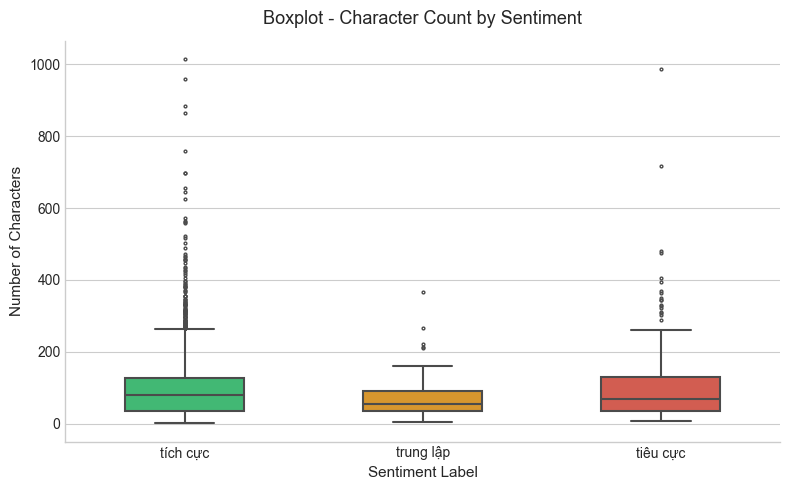
\includegraphics[width=0.9\textwidth]{graphics/boxplot_character_count_by_sentiment.png}
    \caption{Biểu đồ hộp số lượng ký tự theo nhãn cảm xúc.}
    \label{fig:boxplot_character_count_sentiment}
\end{figure}

Quan sát trực quan từ biểu đồ hộp của số lượng ký tự theo nhãn cảm xúc (Hình~\ref{fig:boxplot_character_count_sentiment}) cũng cho thấy khác biệt rõ ở phần đuôi phân phối. Mặc dù phần lớn bình luận của cả ba nhóm đều tập trung dưới ngưỡng 200 ký tự, nhóm tiêu cực có dải phân tán rộng hơn và xuất hiện nhiều ngoại lai ở vùng giá trị rất cao; một số mẫu vượt xa mốc 700 đến gần 1.000 ký tự. Ngược lại, nhóm trung lập có phân bố hẹp hơn, ít biến động và số lượng ngoại lai thấp hơn đáng kể, phản ánh xu hướng để lại nhận xét ngắn, trực tiếp và ít diễn giải.

\vspace{0.5em}
\noindent\textcolor{lightblue}{\textbf{Kiểm định Mann--Whitney U}}\par
\vspace{0.5em}
Để kiểm chứng một cách chặt chẽ giả thuyết rằng bình luận tiêu cực có xu hướng dài hơn bình luận tích cực, nhóm nghiên cứu áp dụng kiểm định phi tham số Mann--Whitney U trên phân phối số từ giữa hai nhóm. Việc lựa chọn kiểm định này là cần thiết vì phân phối độ dài văn bản bị lệch và không thỏa mãn giả định phân phối chuẩn. Kết quả thu được cho thấy thống kê kiểm định đạt $U = 538.779$, giá trị $p$ một phía bằng $0{,}032884$ và hệ số kích thước hiệu ứng đạt $r = 0{,}0271$. Đồng thời, trung vị số từ của nhóm tiêu cực là $15{,}0$, trong khi nhóm tích cực đạt $16{,}0$.

Với mức ý nghĩa $\alpha = 0{,}05$, giá trị $p < 0{,}05$ cho phép bác bỏ giả thuyết không, qua đó xác nhận rằng phân phối độ dài giữa hai nhóm có khác biệt về mặt thống kê. Tuy nhiên, cần nhấn mạnh rằng khác biệt này chủ yếu đến từ phần đuôi phân phối của nhóm tiêu cực --- nơi xuất hiện nhiều bình luận rất dài --- chứ không phản ánh sự chênh lệch lớn ở phần trung tâm của toàn bộ dữ liệu.

\vspace{0.5em}
\noindent\textcolor{lightblue}{\textbf{Kết luận thống kê}}\par
\vspace{0.5em}
Từ góc nhìn thực tiễn, mặc dù kiểm định cho kết quả có ý nghĩa thống kê, hệ số kích thước hiệu ứng $r = 0{,}0271$ là cực nhỏ và trung vị giữa hai nhóm gần như tương đương nhau. Điều này cho thấy đối với phần lớn bình luận thông thường, độ dài văn bản không tạo ra sự phân tách mạnh giữa cảm xúc tích cực và tiêu cực. Nói cách khác, đặc trưng độ dài chỉ mang tín hiệu bổ sung ở các trường hợp ngoại lệ, đặc biệt là những phản hồi tiêu cực có xu hướng mô tả dài và chi tiết hơn mức thông thường.

Do đó, \texttt{word\_count} và \texttt{char\_count} nên được xem là các đặc trưng phụ trợ thay vì đặc trưng quyết định. Khi kết hợp với các biểu diễn nội dung như TF-IDF hoặc vector ngữ nghĩa, nhóm đặc trưng này vẫn có giá trị trong việc bổ sung tín hiệu về cường độ diễn đạt, nhưng không đủ mạnh để sử dụng độc lập như nền tảng chính cho mô hình phân loại cảm xúc.

\subsubsection{Phân tích từ vựng}

\vspace{0.5em}
\noindent\textcolor{lightblue}{\textbf{Trực quan hóa đám mây từ vựng}}\par
\vspace{0.5em}
Trực quan hóa các từ vựng xuất hiện phổ biến nhất của các nhóm bình luận tích cực, trung lập và tiêu cực dưới dạng đám mây từ vựng giúp nhận diện nhanh những từ khóa trọng tâm cũng như khác biệt tổng quan về mặt ngữ nghĩa giữa các nhóm cảm xúc.

\begin{figure}[H]
    \centering
    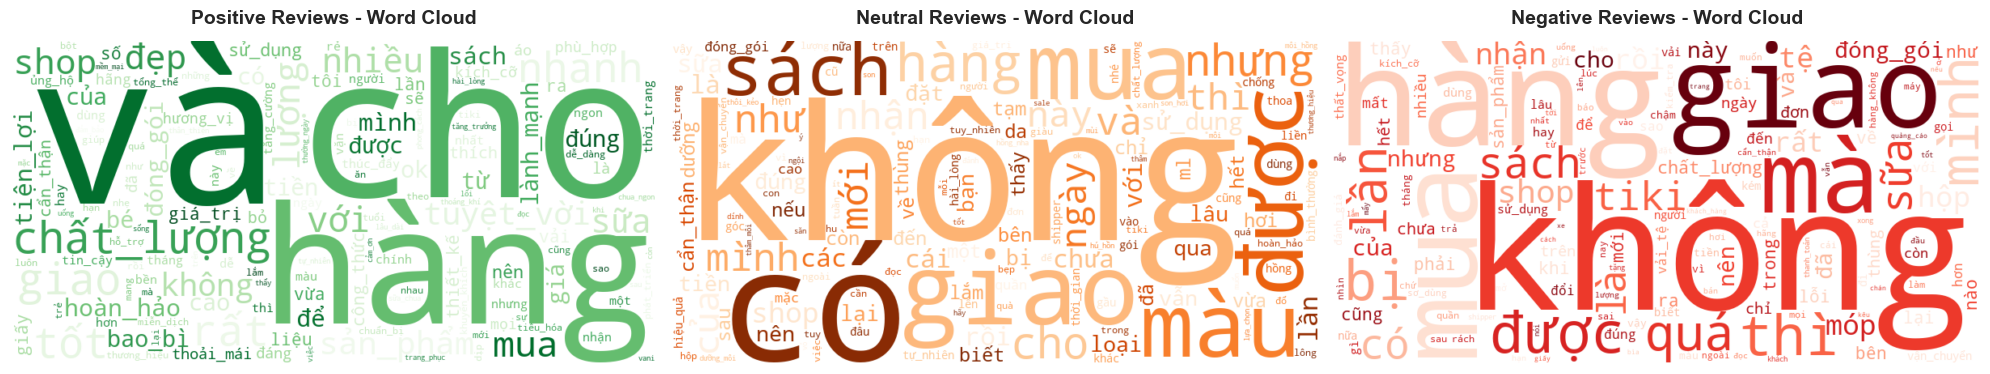
\includegraphics[width=\textwidth]{graphics/wordcloud_sentiment_groups.png}
    \caption{Đám mây từ vựng của ba nhóm cảm xúc: tích cực, trung lập và tiêu cực.}
    \label{fig:wordcloud_sentiment_groups}
\end{figure}

Nhận xét từ Hình~\ref{fig:wordcloud_sentiment_groups} có thể tóm lược như sau:

\begin{itemize}[labelsep=10pt, leftmargin=2cm]
    \item \textbf{Nhóm tích cực:} nổi bật với các từ khóa mang sắc thái khen ngợi rõ ràng như ``chất\_lượng'', ``tốt'', ``đẹp'', ``nhanh''. Điều này cho thấy người dùng chủ yếu bày tỏ sự hài lòng về chất lượng sản phẩm và tốc độ giao hàng.
    \item \textbf{Nhóm trung lập:} xuất hiện nhiều từ mang tính kể lể hoặc cấu trúc tương phản như ``nhưng'', ``không'', ``có''. Điều này cho thấy các đánh giá trung lập thường chứa cả yếu tố khen lẫn chê, phản ánh thái độ chấp nhận ở mức vừa phải.
    \item \textbf{Nhóm tiêu cực:} bị áp đảo bởi các từ chỉ sự cố và thái độ thất vọng như ``không'', ``bị'', ``tệ'', ``quá'', ``móp''. Khách hàng trong nhóm này tập trung phản ánh tình trạng hàng hóa lỗi hoặc trải nghiệm dịch vụ không đạt kỳ vọng.
\end{itemize}

\vspace{0.5em}
\noindent\textcolor{lightblue}{\textbf{Phân tích n-gram theo nhóm cảm xúc}}\par
\vspace{0.5em}
Phân tích top 20 unigram, bigram và trigram theo từng nhóm cảm xúc giúp bộc lộ các cụm từ đặc trưng mà phân tích đơn lẻ từng từ không thể nắm bắt được. Nhóm sử dụng \texttt{TfidfVectorizer} với \texttt{use\_idf=False} để đo tần suất thuần, tức chỉ xét tần suất xuất hiện của từ mà không điều chỉnh theo trọng số IDF.

\begin{figure}[H]
    \centering
    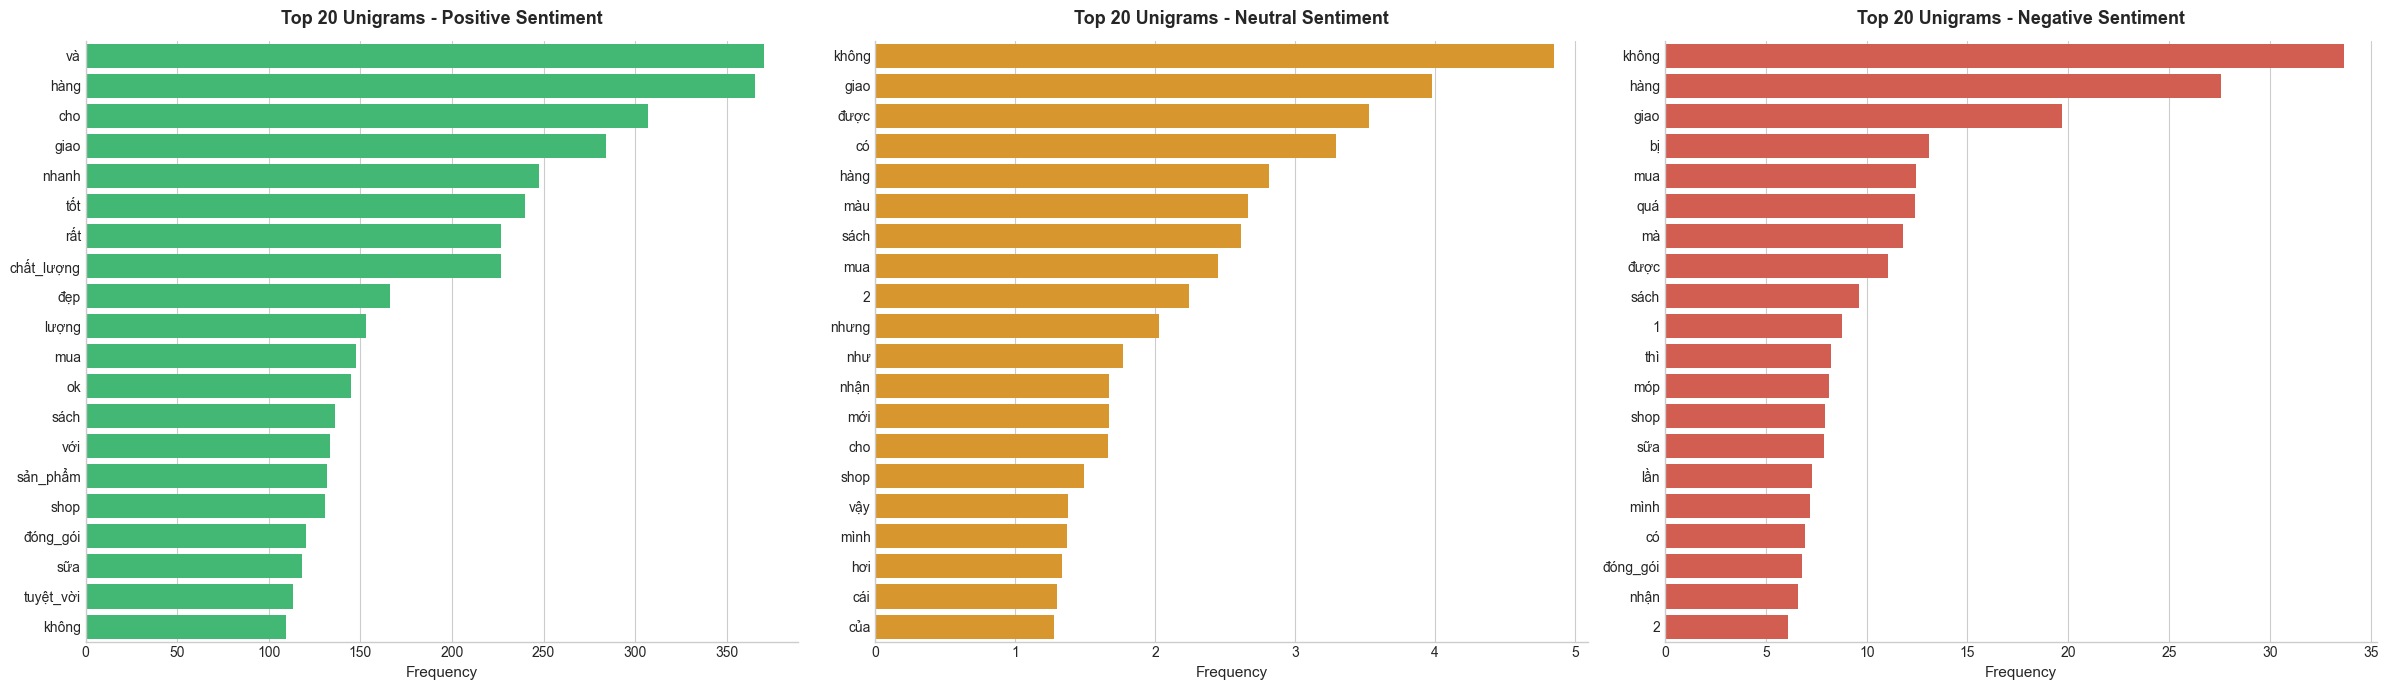
\includegraphics[width=\textwidth]{graphics/ngram_unigram_top20.png}
    \caption{Top 20 unigram theo ba nhóm cảm xúc: tích cực, trung lập và tiêu cực.}
    \label{fig:ngram_unigram_top20}
\end{figure}

\begin{figure}[H]
    \centering
    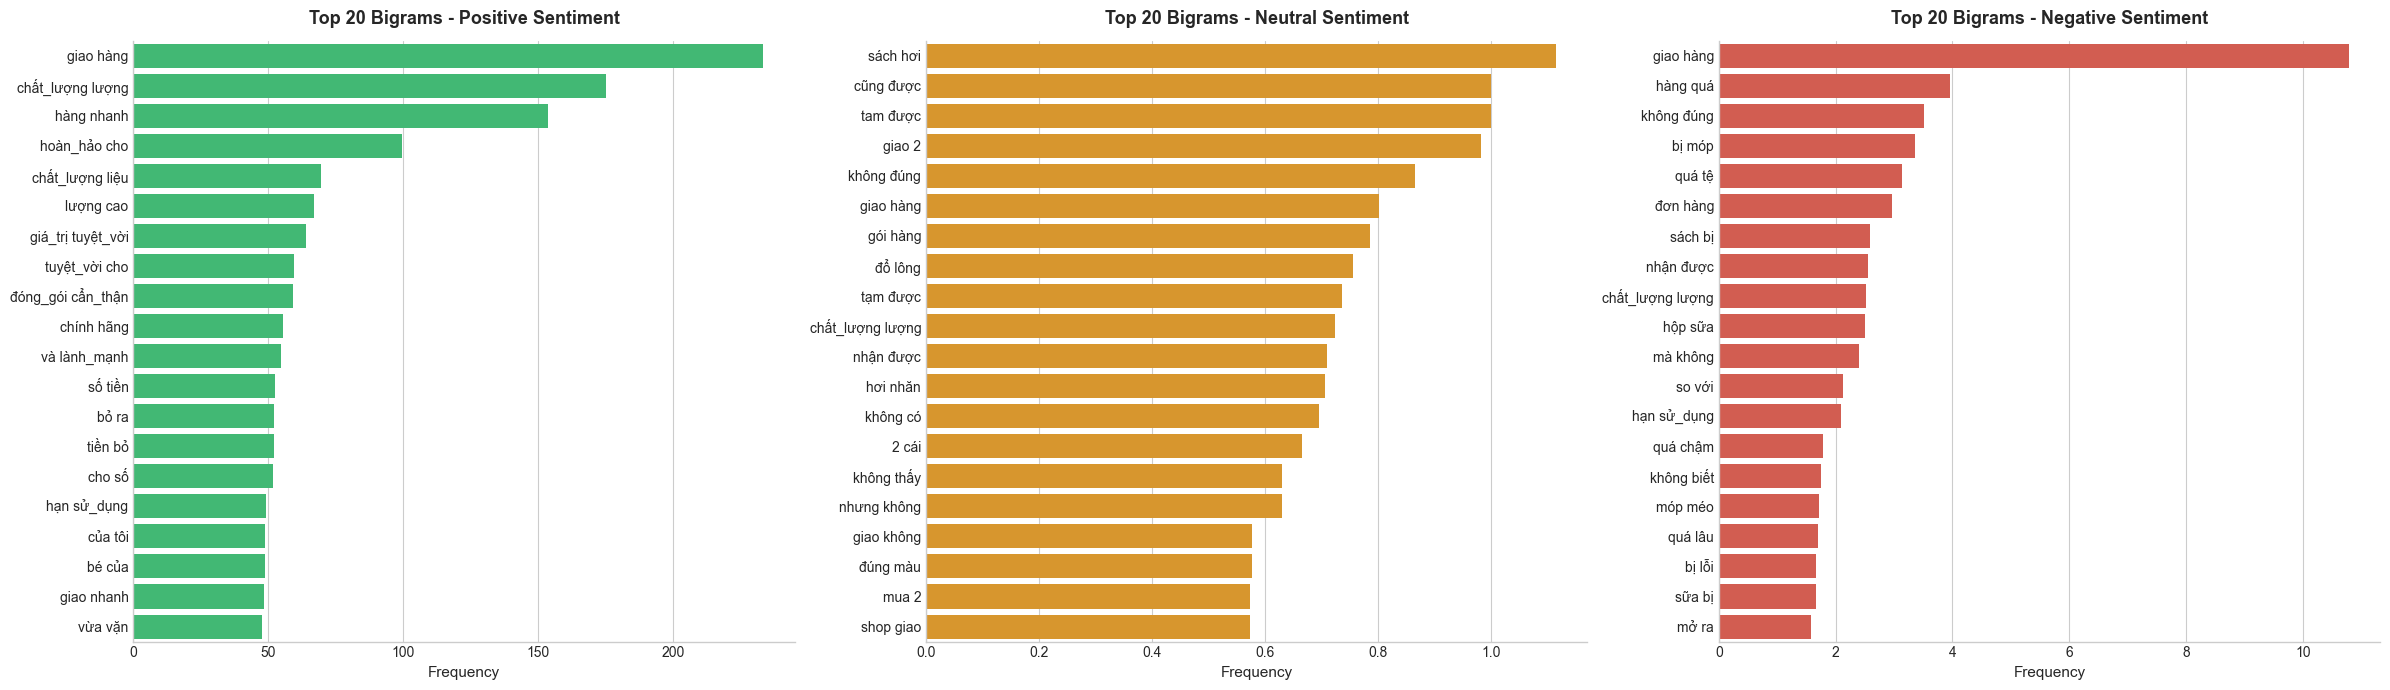
\includegraphics[width=\textwidth]{graphics/ngram_bigram_top20.png}
    \caption{Top 20 bigram theo ba nhóm cảm xúc: tích cực, trung lập và tiêu cực.}
    \label{fig:ngram_bigram_top20}
\end{figure}

\begin{figure}[H]
    \centering
    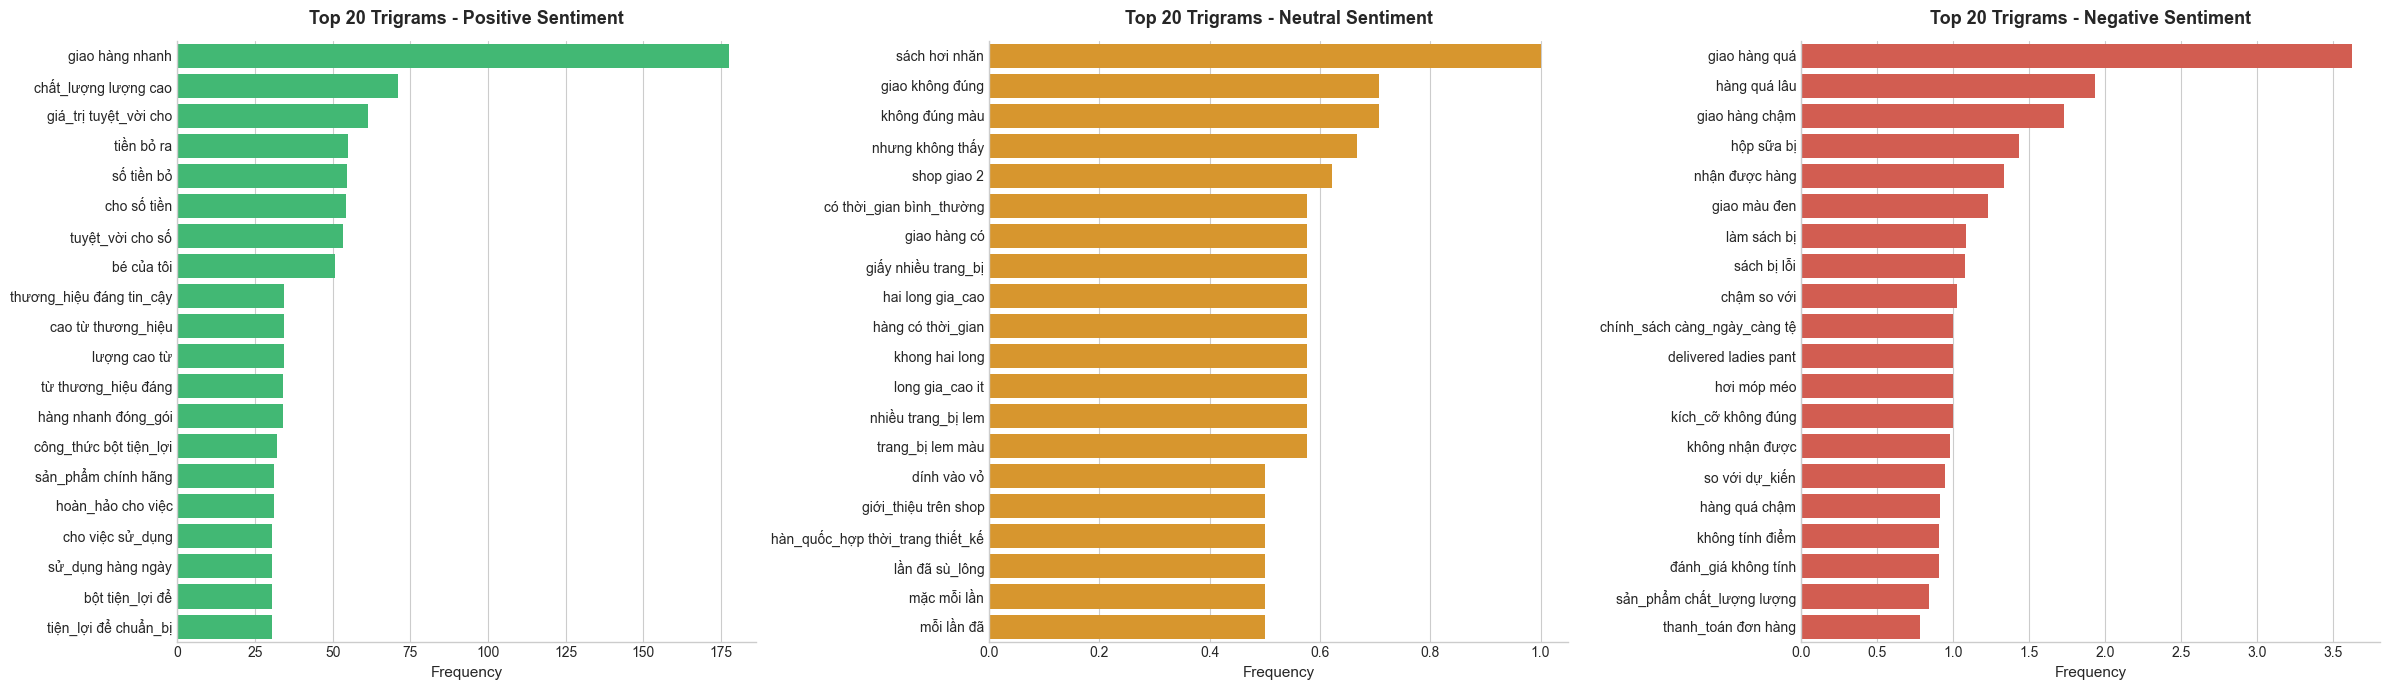
\includegraphics[width=\textwidth]{graphics/ngram_trigram_top20.png}
    \caption{Top 20 trigram theo ba nhóm cảm xúc: tích cực, trung lập và tiêu cực.}
    \label{fig:ngram_trigram_top20}
\end{figure}

Kết quả phân tích có thể được tóm lược như sau:

\begin{itemize}[labelsep=10pt, leftmargin=2cm]
    \item Ở cấp độ unigram, cả ba nhóm đều chứa các từ chung như ``hàng'' và ``giao'', do đó khả năng phân biệt sắc thái cảm xúc còn hạn chế.
    \item Khi chuyển sang bigram, ngữ cảnh đánh giá trở nên rõ ràng hơn đáng kể: nhóm tích cực thường gắn với các cụm như ``giao hàng nhanh'' và ``chất lượng tốt'', trong khi nhóm tiêu cực nổi bật với các biểu thức như ``giao hàng chậm'', ``bị móp'' hoặc ``không đúng''. Đối với nhóm trung lập, các cụm ``cũng được'' và ``tạm ổn'' phản ánh thái độ chấp nhận ở mức vừa phải.
    \item Ở cấp độ trigram, các tín hiệu ngữ nghĩa tiếp tục được củng cố. Những cụm như ``giao hàng quá lâu'' hoặc ``sách bị lỗi'' là các dấu hiệu phân biệt rất mạnh cho nhóm tiêu cực.
    \item Từ các quan sát trên, có thể kết luận rằng việc sử dụng cấu hình \texttt{ngram\_range=(1,\,2)} hoặc \texttt{(1,\,3)} trong bước vector hóa là cần thiết để thu thập được các tín hiệu ngôn ngữ phức hợp, thay vì chỉ dựa vào các từ đơn lẻ.
\end{itemize}

\vspace{0.5em}
\noindent\textcolor{lightblue}{\textbf{Tỷ lệ loại trên tổng số từ}}\par
\vspace{0.5em}
Tỷ lệ loại trên tổng số từ đo lường mức độ phong phú của từ vựng trong từng nhóm cảm xúc, được xác định bằng tỉ số giữa số lượng từ duy nhất và tổng số từ xuất hiện. Giá trị càng cao cho thấy ngôn ngữ càng đa dạng; ngược lại, giá trị thấp phản ánh xu hướng lặp lại khuôn mẫu diễn đạt.

\begin{center}
\renewcommand{\arraystretch}{1.4}
\begin{tabularx}{\textwidth}{|l|c|c|c|}
\hline
\rowcolor[HTML]{E8E8E8}
\textbf{Nhóm cảm xúc} & \textbf{Tổng số từ} & \textbf{Số từ duy nhất} & \textbf{Tỷ lệ loại trên tổng số từ} \\
\hline
Tích cực & $> 79.000$ & $\approx 4.400$ & $0{,}0560$ \\
\hline
Tiêu cực & $\approx 9.000$ & $\approx 1.900$ & $0{,}2076$ \\
\hline
Trung lập & $\approx 823$ & $\approx 385$ & $0{,}4678$ \\
\hline
\end{tabularx}
\captionof{table}{\centering Tỷ lệ loại trên tổng số từ theo nhóm cảm xúc}
\end{center}

Kết quả cho thấy nhóm tích cực có tỷ lệ thấp nhất dù quy mô dữ liệu lớn nhất, chứng tỏ các bình luận khen ngợi thường sử dụng một tập từ vựng khá lặp lại như ``tốt'', ``đẹp'', ``ok'', ``nhanh''. Ngược lại, nhóm tiêu cực có tỷ lệ cao hơn rõ rệt, phản ánh xu hướng dùng ngôn ngữ phong phú và chi tiết hơn để mô tả lỗi hoặc trải nghiệm không hài lòng. Đối với nhóm trung lập, giá trị cao nhất chủ yếu chịu ảnh hưởng bởi kích thước mẫu nhỏ; theo định luật Heap, tập dữ liệu càng nhỏ thì chỉ số này càng dễ tăng cao, do đó cần thận trọng khi diễn giải.

\vspace{0.5em}
\noindent\textcolor{lightblue}{\textbf{Kiểm chứng định luật Zipf}}\par
\vspace{0.5em}
Định luật Zipf phát biểu rằng tần suất của một từ tỷ lệ nghịch với thứ hạng của nó trên đồ thị log--log. Việc kiểm chứng quy luật này trên toàn bộ tập văn bản giúp đánh giá mức độ tự nhiên của ngôn ngữ và nhận diện vùng từ hiếm trước khi xây dựng ma trận đặc trưng.

\begin{figure}[H]
    \centering
    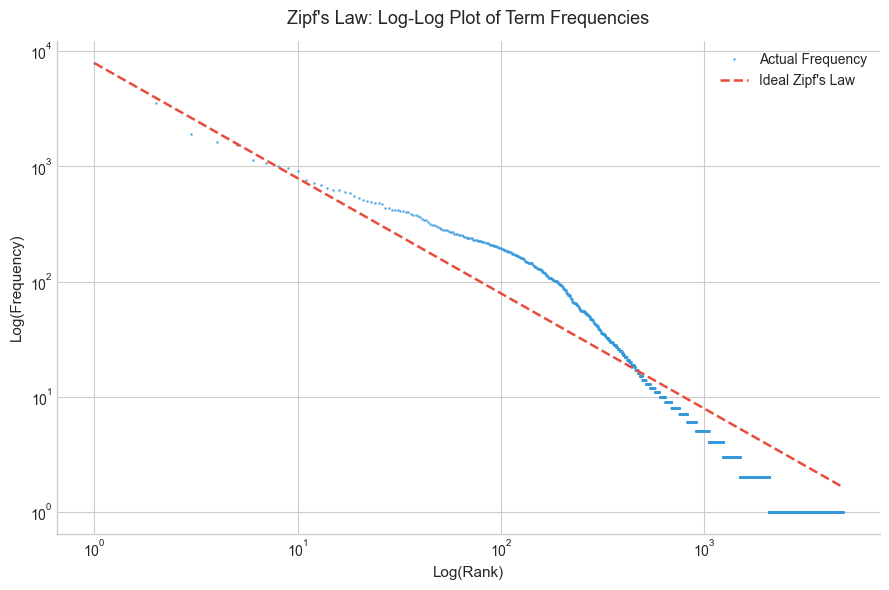
\includegraphics[width=0.9\textwidth]{graphics/zipf_kiem_chung.png}
    \caption{Kiểm chứng định luật Zipf trên tập văn bản đánh giá.}
    \label{fig:zipf_kiem_chung}
\end{figure}

Kết quả cho thấy đường quan sát bám khá sát đường Zipf lý tưởng ở phần đầu phân phối, xác nhận rằng tập dữ liệu tuân theo quy luật tự nhiên của ngôn ngữ con người và không bị chi phối bởi văn bản sinh ngẫu nhiên hay nhiễu bất thường. Ở dải thứ hạng từ 10 đến 100, đường quan sát nhô lên so với đường lý thuyết, phản ánh đặc điểm chuyên ngành của dữ liệu thương mại điện tử khi các từ như ``giao'', ``hàng'', ``chất lượng'' hay ``shop'' được lặp lại với tần suất cao hơn ngôn ngữ thông thường. Ở phần đuôi, đường cong giảm rất nhanh và tạo thành các bậc thang, cho thấy sự hiện diện của số lượng lớn từ hiếm chỉ xuất hiện một hoặc hai lần --- thường là lỗi chính tả, từ viết tắt bất thường hoặc tên sản phẩm đặc thù. Điều này củng cố sự cần thiết của việc thiết lập tham số \texttt{min\_df} trong bước vector hóa nhằm loại bỏ các từ quá hiếm và tránh làm ma trận TF-IDF phình to không cần thiết.

\subsubsection{Biểu diễn đặc trưng thưa --- TF-IDF}

Biểu diễn đặc trưng thưa bằng TF-IDF là một phương pháp kinh điển trong xử lý ngôn ngữ tự nhiên. Cách tiếp cận này biến đổi tập văn bản thành một không gian véc-tơ dựa trên tần suất xuất hiện tương đối của từ hoặc cụm từ n-gram, đồng thời làm giảm ảnh hưởng của các đơn vị ngôn ngữ xuất hiện quá phổ biến trong toàn bộ tập dữ liệu. Kết quả thu được là một ma trận dạng \texttt{(số tài liệu $\times$ số đặc trưng)} mà phần lớn các phần tử có giá trị bằng 0, qua đó phản ánh đúng bản chất thưa của dữ liệu văn bản sau vector hóa.

\vspace{0.5em}
\noindent\textcolor{lightblue}{\textbf{Vector hóa TF-IDF}}\par
\vspace{0.5em}
Ở bước này, nhóm nghiên cứu khởi tạo và huấn luyện bộ biến đổi TF-IDF để chuyển tập đánh giá thành ma trận đặc trưng thưa. Quá trình này đồng thời kiểm soát số chiều của không gian biểu diễn và loại bỏ các từ quá hiếm thông qua các tham số như \texttt{min\_df} và \texttt{max\_features}, nhằm cân bằng giữa khả năng biểu diễn nội dung và chi phí tính toán.

\begin{center}
\renewcommand{\arraystretch}{1.4}
\begin{tabularx}{0.75\textwidth}{|X|c|}
\hline
\rowcolor[HTML]{E8E8E8}
\textbf{Thuộc tính} & \textbf{Giá trị} \\
\hline
Kích thước ma trận (tài liệu $\times$ đặc trưng) & $4.651 \times 4.408$ \\
\hline
Số phần tử khác 0 & $102.320$ \\
\hline
Tỷ lệ thưa thớt & $99,50\%$ \\
\hline
Bộ nhớ sử dụng & $0,82$ MB \\
\hline
\end{tabularx}
\captionof{table}{\centering Các thuộc tính chính của ma trận TF-IDF}
\end{center}

Các thông số trên cho thấy ma trận đặc trưng sau vector hóa có mức độ thưa thớt rất cao, với chỉ khoảng $0,5\%$ số phần tử khác 0. Đây là đặc điểm điển hình của biểu diễn TF-IDF trên dữ liệu đánh giá ngắn, nơi mỗi văn bản chỉ kích hoạt một tập nhỏ đặc trưng trong toàn bộ từ vựng. Dung lượng bộ nhớ chỉ ở mức $0,82$ MB cho thấy biểu diễn này vẫn khá gọn nhẹ, phù hợp cho các mô hình học máy tuyến tính và các bước phân tích không gian đặc trưng tiếp theo.

\vspace{0.5em}
\noindent\textcolor{lightblue}{\textbf{Trực quan hóa t-SNE}}\par
\vspace{0.5em}
Nhóm nghiên cứu tiếp tục áp dụng thuật toán giảm chiều t-SNE để chiếu không gian TF-IDF xuống mặt phẳng hai chiều. Bước này giúp trực quan hóa hình học của không gian đặc trưng và đánh giá xem các nhóm cảm xúc có thực sự phân tách thành các cụm riêng biệt hay không.

\begin{figure}[H]
    \centering
    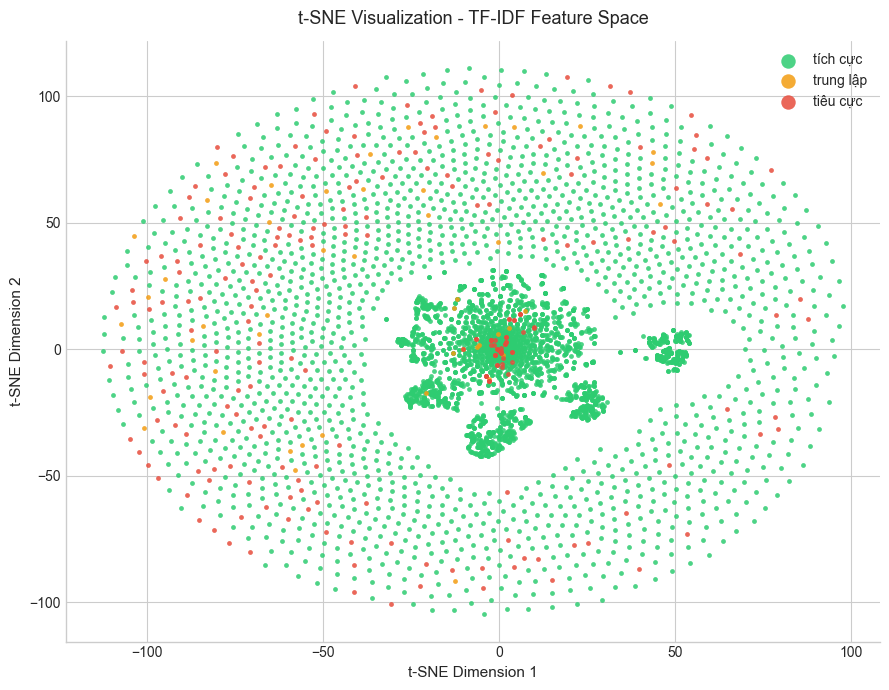
\includegraphics[width=0.92\textwidth]{graphics/tsne_tfidf_feature_space.png}
    \caption{Trực quan hóa t-SNE không gian đặc trưng TF-IDF theo ba nhóm cảm xúc.}
    \label{fig:tsne_tfidf_feature_space}
\end{figure}

Nhận xét từ biểu đồ t-SNE trong Hình~\ref{fig:tsne_tfidf_feature_space} có thể được tóm lược như sau:

\begin{itemize}[labelsep=10pt, leftmargin=2cm]
    \item \textbf{Bị chi phối bởi dữ liệu mất cân bằng:} lớp tích cực chiếm số lượng áp đảo và phủ gần như toàn bộ không gian phân phối. Điều này phản ánh đúng tình trạng mất cân bằng nhãn của tập dữ liệu gốc, trong đó phần lớn đánh giá thuộc nhóm tích cực.
    \item \textbf{Ranh giới phân loại chồng lấp mạnh:} các điểm tiêu cực và trung lập phân tán rải rác, đồng thời trộn lẫn đáng kể vào đám mây điểm tích cực. Chúng không hình thành các cụm độc lập, tách biệt rõ ràng trong không gian hai chiều.
    \item \textbf{Hạn chế của biểu diễn TF-IDF:} sự chồng lấp trên cho thấy TF-IDF chủ yếu gom nhóm dựa trên sự xuất hiện của các từ vựng bề mặt phổ biến như ``hàng'', ``giao'', ``shop'' mà chưa đủ khả năng tách bạch các sắc thái ngữ nghĩa sâu hơn. Điều này dự báo rằng các mô hình phân loại tuyến tính cơ bản sẽ gặp khó khăn khi phải xác định ranh giới quyết định chính xác, đặc biệt đối với các lớp thiểu số.
\end{itemize}

\subsubsection{Biểu diễn ngữ nghĩa dày đặc --- Vietnamese SBERT}

Trái ngược với biểu diễn TF-IDF vốn chủ yếu dựa trên tần suất bề mặt của từ vựng, biểu diễn ngữ nghĩa dày đặc hướng tới việc bảo toàn ngữ nghĩa sâu của câu thông qua các mô hình biến áp câu. Trong nghiên cứu này, nhóm sử dụng mô hình \texttt{keepitreal/vietnamese-sbert} để mã hóa mỗi bình luận thành một véc-tơ có số chiều cố định nhưng chứa hàm lượng thông tin ngữ nghĩa cao. Trong không gian này, các câu có ý nghĩa tương đồng có xu hướng nằm gần nhau về mặt hình học, ngay cả khi chúng không chia sẻ cùng từ vựng bề mặt.

\vspace{0.5em}
\noindent\textcolor{lightblue}{\textbf{Mã hóa bằng Vietnamese SBERT}}\par
\vspace{0.5em}
Nhóm nghiên cứu sử dụng mô hình SBERT chuyên biệt cho tiếng Việt để chuyển đổi toàn bộ tập bình luận thành các véc-tơ nhúng dày đặc. Khác với TF-IDF chỉ đếm số lần xuất hiện của từ khóa, SBERT có khả năng nắm bắt ngữ cảnh và mức độ tương đồng ngữ nghĩa giữa các câu, kể cả trong trường hợp cách diễn đạt khác nhau nhưng nội dung tương đương.

\begin{center}
\renewcommand{\arraystretch}{1.4}
\begin{tabularx}{0.7\textwidth}{|X|c|}
\hline
\rowcolor[HTML]{E8E8E8}
\textbf{Thuộc tính} & \textbf{Giá trị} \\
\hline
Kích thước ma trận nhúng dày đặc & $(4.651,\ 768)$ \\
\hline
Số tài liệu $\times$ số chiều & $4.651 \times 768$ \\
\hline
Bộ nhớ sử dụng & $14,3$ MB \\
\hline
\end{tabularx}
\captionof{table}{\centering Các thuộc tính chính của ma trận nhúng ngữ nghĩa dày đặc}
\end{center}

Kích thước ma trận cho thấy mỗi bình luận được ánh xạ vào một véc-tơ 768 chiều, tạo thành không gian đặc trưng dày đặc có khả năng biểu diễn nội dung ở mức ngữ nghĩa thay vì chỉ ở mức từ vựng rời rạc. Mặc dù dung lượng bộ nhớ tăng lên so với biểu diễn TF-IDF, chi phí này đổi lại khả năng mã hóa tốt hơn các quan hệ ngữ nghĩa giữa các câu, từ đó mở ra tiềm năng phân tách lớp hiệu quả hơn trong các bước trực quan hóa và mô hình hóa tiếp theo.

\vspace{0.5em}
\noindent\textcolor{lightblue}{\textbf{Trực quan hóa t-SNE trên không gian dày đặc}}\par
\vspace{0.5em}
Sau khi thu được ma trận nhúng ngữ nghĩa, nhóm tiếp tục áp dụng thuật toán t-SNE để giảm chiều không gian dày đặc xuống hai chiều nhằm phục vụ trực quan hóa. Việc đối chiếu biểu đồ này với biểu đồ t-SNE của TF-IDF sẽ giúp đánh giá liệu biểu diễn SBERT có thực sự kéo các bình luận cùng sắc thái cảm xúc lại gần nhau hơn và tách các nhóm tốt hơn hay không.

\begin{figure}[H]
    \centering
    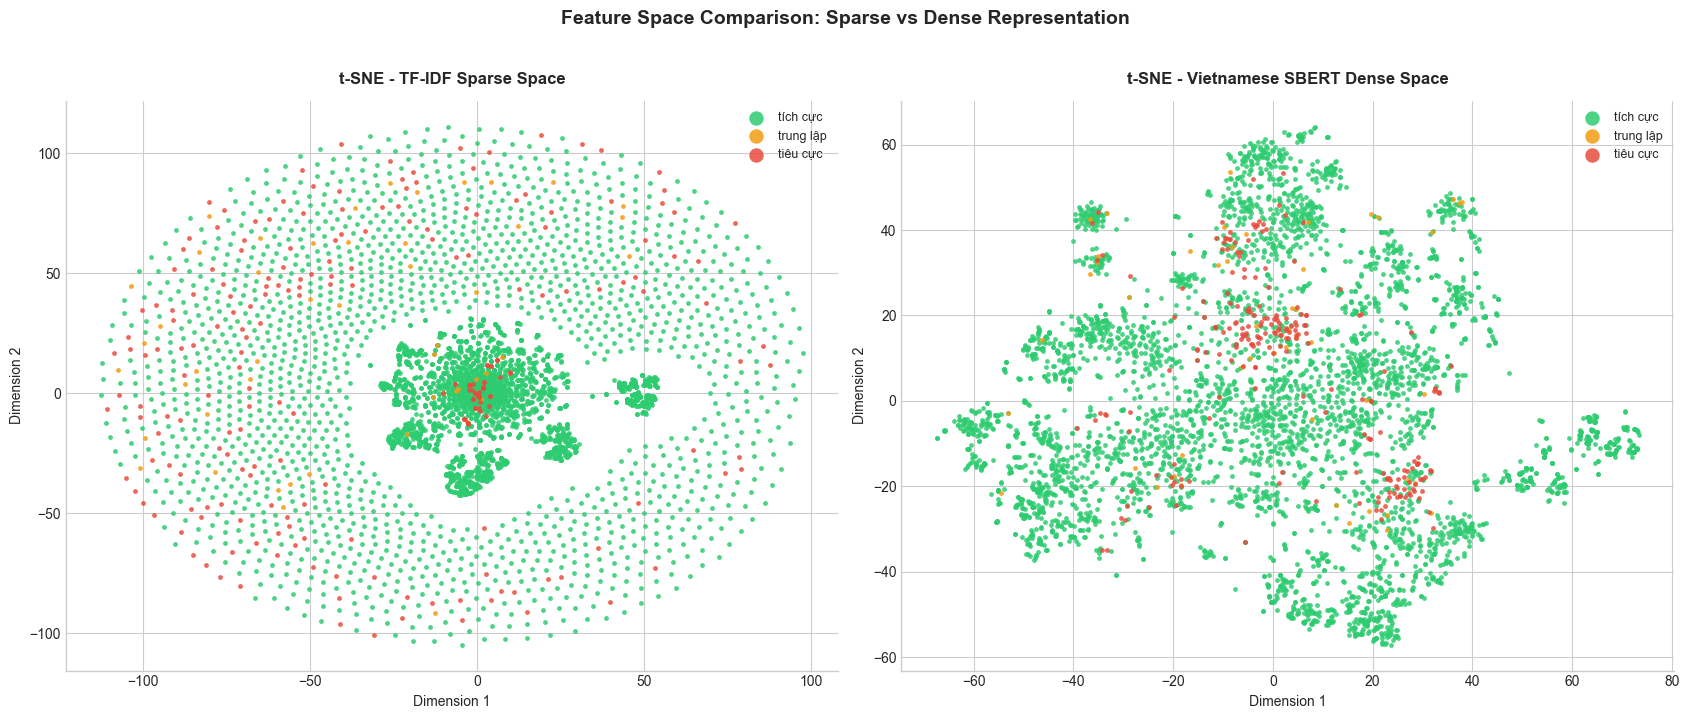
\includegraphics[width=\textwidth]{graphics/compare_tfidf_sbert_tsne.png}
    \caption{So sánh trực quan không gian đặc trưng TF-IDF và Vietnamese SBERT sau khi giảm chiều bằng t-SNE.}
    \label{fig:compare_tfidf_sbert_tsne}
\end{figure}

Nhận xét khi so sánh hai không gian đặc trưng trong Hình~\ref{fig:compare_tfidf_sbert_tsne} có thể được tóm lược như sau:

\begin{itemize}[labelsep=10pt, leftmargin=2cm]
    \item \textbf{Hình thái phân bố:} biểu đồ TF-IDF tạo ra một cấu trúc hình khuyên khá nhân tạo với lõi đặc và viền thưa, vốn là một dạng hiện tượng thường gặp khi áp dụng t-SNE trên dữ liệu quá thưa. Ngược lại, không gian SBERT phân bố tự nhiên và hữu cơ hơn, hình thành nhiều cụm nhỏ mang ý nghĩa ngữ nghĩa rõ ràng hơn.
    \item \textbf{Khả năng gom nhóm:} trong không gian TF-IDF, các điểm tiêu cực và trung lập rải rác khá ngẫu nhiên và bị hòa lẫn mạnh vào lớp tích cực. Khi chuyển sang không gian dày đặc của SBERT, các điểm tiêu cực bắt đầu có xu hướng co cụm tại một số vùng cục bộ, cho thấy biểu diễn ngữ nghĩa đã giữ lại được tín hiệu cấu trúc tốt hơn.
    \item \textbf{Kết luận trực quan:} mặc dù hiện tượng chồng lấp vẫn tồn tại do tập dữ liệu mất cân bằng nặng, biểu đồ cho thấy SBERT đã nắm bắt tốt hơn các tương đồng ngữ nghĩa sâu xa và kéo các bình luận có nội dung gần nhau lại gần hơn so với phương pháp đếm từ khóa bề mặt như TF-IDF.
\end{itemize}

\subsubsection{Thử nghiệm gom cụm K-Means không giám sát}

Nhóm nghiên cứu tiến hành thử nghiệm thuật toán gom cụm K-Means với số cụm $k=3$ trên không gian nhúng ngữ nghĩa của SBERT mà không sử dụng trước nhãn cảm xúc. Mục tiêu của phép thử này là đánh giá xem cấu trúc hình học của không gian SBERT có đủ mạch lạc để tự hình thành các cụm tự nhiên hay không, từ đó cung cấp thêm bằng chứng về chất lượng biểu diễn ngữ nghĩa dày đặc.

\begin{figure}[H]
    \centering
    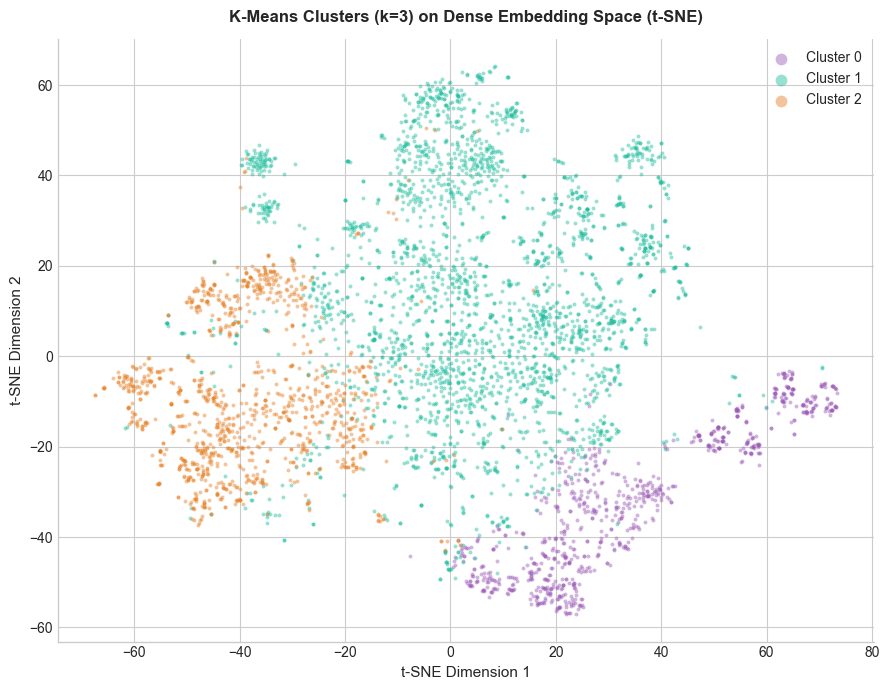
\includegraphics[width=0.92\textwidth]{graphics/kmeans_sbert_tsne.png}
    \caption{Các cụm K-Means $(k=3)$ trên không gian nhúng SBERT sau khi giảm chiều bằng t-SNE.}
    \label{fig:kmeans_sbert_tsne}
\end{figure}

Nhận xét từ kết quả gom cụm trong Hình~\ref{fig:kmeans_sbert_tsne} có thể được tóm lược như sau:

\begin{itemize}[labelsep=10pt, leftmargin=2cm]
    \item \textbf{Phân cụm rõ nét:} dù không được cung cấp nhãn cảm xúc từ trước, thuật toán K-Means vẫn tự động chia không gian SBERT thành ba cụm hình học tương đối tách biệt. Điều này cho thấy không gian đặc trưng dày đặc sở hữu cấu trúc toán học đủ ổn định để hỗ trợ các phương pháp học không giám sát.
    \item \textbf{Gom cụm theo chủ đề ngữ nghĩa:} do dữ liệu tích cực chiếm tỷ trọng áp đảo, ba cụm thu được không nhất thiết tương ứng hoàn toàn với ba nhãn cảm xúc, mà nhiều khả năng phản ánh ba chủ đề ngữ nghĩa tự nhiên trong đánh giá của khách hàng, chẳng hạn như khen giao hàng, khen sản phẩm hoặc phản ánh vấn đề phát sinh.
    \item \textbf{Ưu thế của SBERT:} kết quả trực quan này củng cố nhận định rằng SBERT vượt trội hơn TF-IDF trong việc nắm bắt quan hệ ngữ nghĩa sâu. Nhờ đó, biểu diễn này đặc biệt phù hợp làm đầu vào cho các mô hình học sâu hoặc các chiến lược học biểu diễn nâng cao ở giai đoạn tiếp theo.
\end{itemize}

\subsection{Khám phá chuyên sâu đặc trưng dữ liệu hình ảnh ngoại tuyến}
% Nội dung đồng đội cần viết:
% - Thống kê chất lượng hình ảnh: trực quan hóa phân bố độ phân giải và giá trị phân bố điểm ảnh của tập dữ liệu thị giác.
% - Phân tích đặc tính thị giác: khảo sát độ sáng tối trung bình và độ tương phản giữa các nhóm nhãn hình ảnh khác nhau nhằm nhận diện ngoại lệ (ảnh quá mờ hoặc lóa).
% - Kiểm tra chất lượng nâng cao: ứng dụng thuật toán băm cảm nhận để quét và định lượng tỷ lệ trùng lặp hình ảnh, phát hiện các trường hợp mượn ảnh từ nguồn khác để đánh giá.
\label{sec:phan_tich_du_lieu_anh}

Phần này trình bày kết quả phân tích khám phá đối với tập ảnh sau bước kiểm
tra chất lượng (Mục~\ref{sec:kiem_tra_du_lieu_anh}), tập trung vào bốn khía
cạnh: phân bố độ phân giải gốc, phân phối cường độ điểm ảnh theo kênh màu,
đặc trưng quang học theo nhãn kết hợp nhận diện ngoại lệ, và phân tích chuyên
sâu về trùng lặp ảnh nhằm phát hiện khả năng gán nhãn sai liên nhãn.

% ─────────────────────────────────────────────────────────────────────────────
\paragraph{Phân bố độ phân giải.}
Quét toàn bộ 7.987 ảnh ở kích thước gốc (không áp dụng resize) cho kết quả
thống kê mô tả được trình bày tại Bảng~\ref{tab:resolution_stats} và trực quan
hóa tại Hình~\ref{fig:resolution_distribution}.

\begin{table}[H]
    \centering
    \caption{Thống kê mô tả độ phân giải gốc của tập dữ liệu hình ảnh}
    \label{tab:resolution_stats}
    \begin{tabular}{lrrr}
        \hline
        \textbf{Chỉ số} & \textbf{Chiều rộng (px)} & \textbf{Chiều cao (px)}
            & \textbf{Tỉ lệ khung hình} \\
        \hline
        Trung bình  &   975,6 & 1.256,1 & 0,8 \\
        Độ lệch chuẩn & 931,5 &   967,3 & 0,4 \\
        Nhỏ nhất    &    85,0 &    51,0 & 0,3 \\
        Phân vị 25  &   360,0 &   640,0 & 0,6 \\
        Trung vị    &   692,0 &   834,0 & 0,7 \\
        Phân vị 75  & 1.080,0 & 1.440,0 & 0,8 \\
        Lớn nhất    & 5.760,0 & 5.712,0 & 6,1 \\
        \hline
    \end{tabular}
\end{table}

\begin{figure}[H]
    \centering
    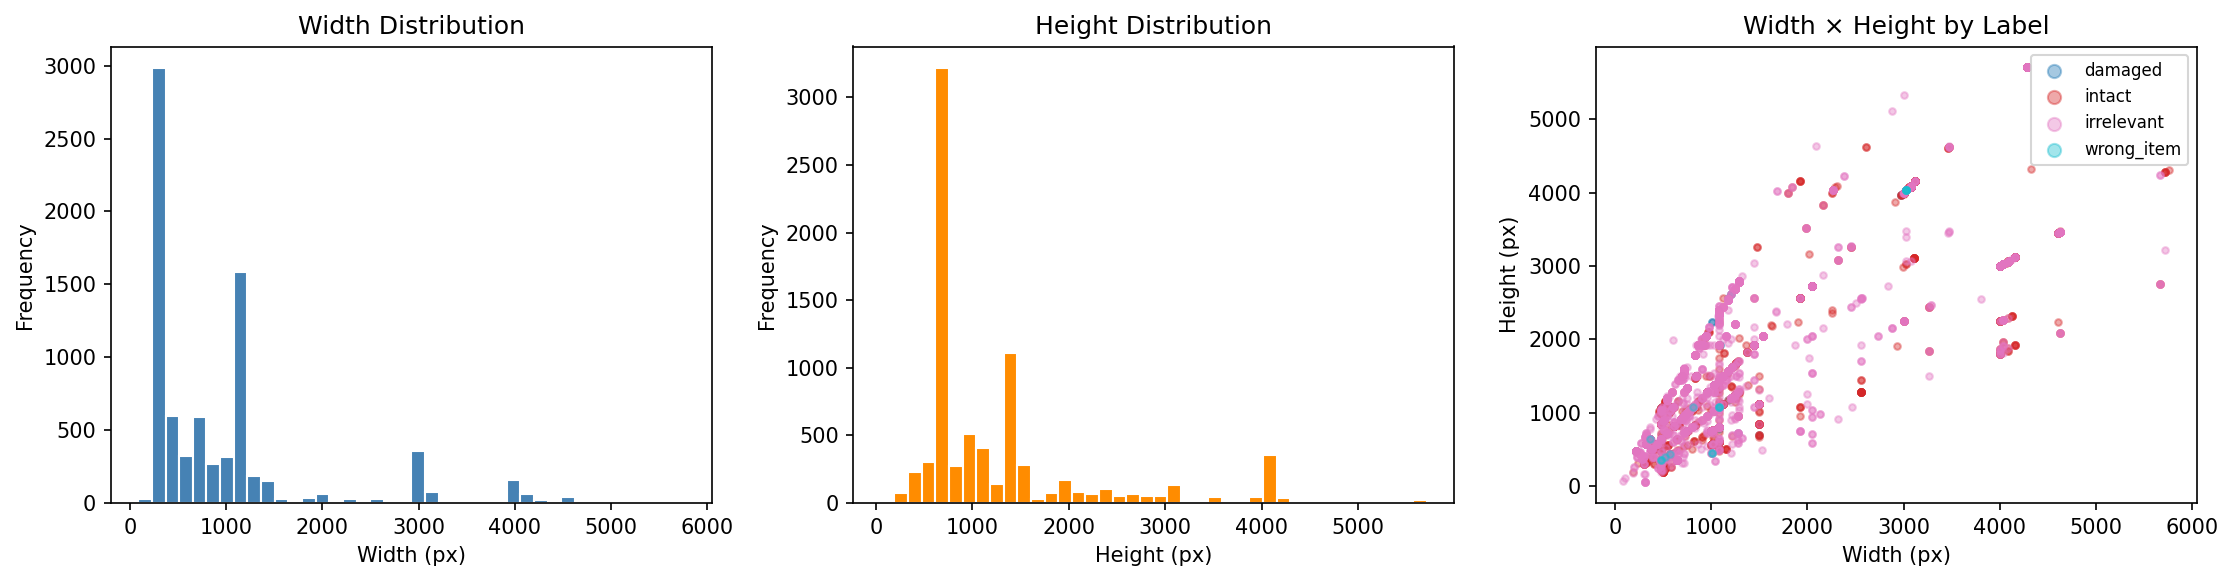
\includegraphics[width=\textwidth]{graphics/resolution_distribution.png}
    \caption{Phân bố chiều rộng, chiều cao và tương quan Width$\times$Height
        theo nhãn của toàn bộ tập dữ liệu.}
    \label{fig:resolution_distribution}
\end{figure}

Phân bố chiều rộng biểu hiện dạng lưỡng đỉnh với cực đại đầu tiên tập trung
quanh 360\,px và cực đại thứ hai quanh 1.080\,px, phản ánh sự tồn tại của hai
nhóm ảnh có nguồn gốc thu thập khác nhau. Phân bố chiều cao tập trung mạnh
quanh 960\,px nhưng có đuôi phải kéo dài đến hơn 5.000\,px, cho thấy một số
ảnh dọc có tỉ lệ khung hình đặc biệt. Biểu đồ tán xạ Width$\times$Height cho
thấy phần lớn mẫu thuộc nhãn \texttt{irrelevant} nằm rải rác trên toàn không
gian độ phân giải, trong khi các nhãn \texttt{damaged} và \texttt{intact} có xu
hướng tập trung hơn. Tổng số ảnh dưới ngưỡng 64$\times$64\,px là 6 mẫu
(0,08\%), toàn bộ thuộc nhãn \texttt{irrelevant}, xác nhận rằng mức độ ảnh có
độ phân giải quá thấp là không đáng kể trong tập dữ liệu.

Độ phân giải trung vị đạt 692$\times$834\,px với tỉ lệ khung hình trung vị 0,7
(ảnh dọc), biện hộ cho ngưỡng resize tối thiểu $64\times64$\,px đã được xác lập
trong bước kiểm tra chất lượng (Mục~\ref{sec:kiem_tra_du_lieu_anh}) và kích
thước làm việc $128\times128$\,px được chọn cho các phân tích nặng.

% ─────────────────────────────────────────────────────────────────────────────
\paragraph{Phân phối cường độ điểm ảnh.}
Phân tích phân phối cường độ điểm ảnh theo từng kênh màu trên tập mẫu 518 ảnh
(Hình~\ref{fig:pixel_distribution}) cho thấy cả ba kênh R, G, B đều biểu hiện
phân phối lưỡng đỉnh: cực đại thứ nhất tập trung ở vùng cường độ thấp (lân cận
0) và cực đại thứ hai nằm trong khoảng cường độ trung bình đến cao
(100\textendash 180). Cấu trúc phân phối này phản ánh sự tồn tại đồng thời của
hai nhóm ảnh có điều kiện chiếu sáng đối lập trong tập dữ liệu và xác nhận sự
cần thiết của bước chuẩn hóa cường độ điểm ảnh trước khi đưa dữ liệu vào mô
hình.

\begin{figure}[H]
    \centering
    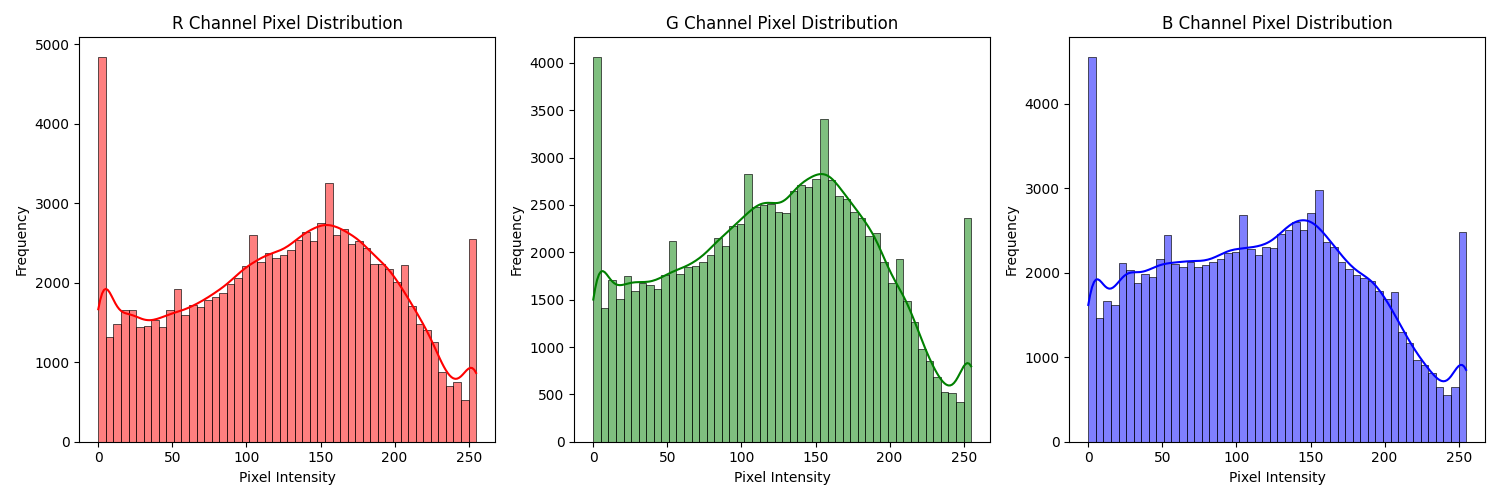
\includegraphics[width=\textwidth]{graphics/pixel_distribution.png}
    \caption{Phân phối cường độ điểm ảnh theo ba kênh màu R, G, B trên tập
        mẫu 518 ảnh.}
    \label{fig:pixel_distribution}
\end{figure}

% ─────────────────────────────────────────────────────────────────────────────
\paragraph{Đặc trưng quang học theo nhãn và nhận diện ngoại lệ.}
Cường độ sáng trung bình và độ tương phản --- đo bằng độ lệch chuẩn cường độ
trên ảnh thang xám --- được tổng hợp theo nhãn tại
Bảng~\ref{tab:brightness_contrast} và Hình~\ref{fig:brightness_contrast}.

\begin{table}[H]
    \centering
    \caption{Cường độ sáng trung bình và độ tương phản theo nhãn}
    \label{tab:brightness_contrast}
    \begin{tabular}{lcc}
        \hline
        \textbf{Nhãn} & \textbf{Cường độ sáng trung bình}
            & \textbf{Độ tương phản (độ lệch chuẩn)} \\
        \hline
        \texttt{damaged}     & 127,87 & 53,38 \\
        \texttt{intact}      & 123,03 & 51,36 \\
        \texttt{irrelevant}  & 116,92 & 45,60 \\
        \texttt{wrong\_item} & 107,30 & 53,58 \\
        \hline
    \end{tabular}
\end{table}

\begin{figure}[H]
    \centering
    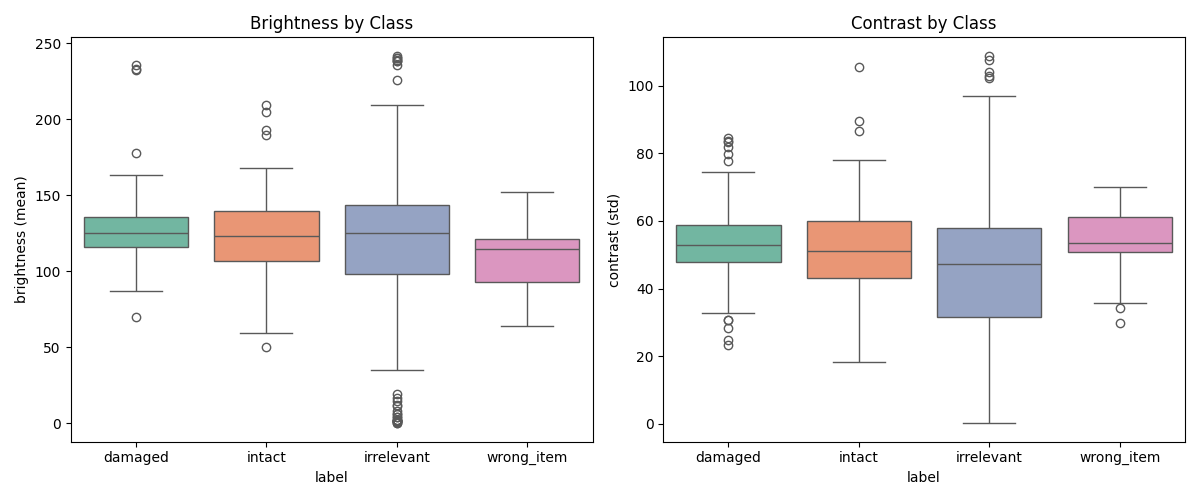
\includegraphics[width=\textwidth]{graphics/brightness_contrast_boxplot.png}
    \caption{Phân bố cường độ sáng và độ tương phản theo nhãn (biểu đồ hộp).}
    \label{fig:brightness_contrast}
\end{figure}

Nhãn \texttt{damaged} ghi nhận cường độ sáng trung bình cao nhất (127,87),
trong khi nhãn \texttt{wrong\_item} có giá trị thấp nhất (107,30). Nhãn
\texttt{irrelevant} có độ tương phản thấp nhất (45,60), phản ánh đặc tính cấu
trúc ảnh đồng nhất hơn so với các nhãn còn lại --- phù hợp với bản chất của
các ảnh không liên quan đến đối tượng sản phẩm cần phân loại.

Áp dụng ngưỡng phát hiện ngoại lệ (cường độ sáng $<50$ hoặc $>200$; độ tương
phản $<20$) trên tập mẫu 518 ảnh phát hiện 49 ảnh ngoại lệ, chiếm 9,5\% tập
mẫu. Bảng~\ref{tab:outlier_summary} trình bày phân bố ngoại lệ theo nhãn và
loại lỗi.

\begin{table}[H]
    \centering
    \caption{Phân bố ảnh ngoại lệ theo nhãn và loại lỗi quang học}
    \label{tab:outlier_summary}
    \begin{tabular}{llc}
        \hline
        \textbf{Nhãn} & \textbf{Loại ngoại lệ} & \textbf{Số lượng} \\
        \hline
        \texttt{damaged}    & Quá sáng (\textit{overexposed})              &  3 \\
        \texttt{intact}     & Độ tương phản thấp (\textit{low\_contrast})  &  1 \\
        \texttt{intact}     & Quá sáng (\textit{overexposed})              &  2 \\
        \texttt{intact}     & Quá tối (\textit{too\_dark})                 &  1 \\
        \texttt{irrelevant} & Độ tương phản thấp (\textit{low\_contrast})  &  3 \\
        \texttt{irrelevant} & Quá sáng (\textit{overexposed})              & 10 \\
        \texttt{irrelevant} & Quá tối (\textit{too\_dark})                 & 10 \\
        \texttt{irrelevant} & Quá tối + Độ tương phản thấp                & 19 \\
        \hline
        \textbf{Tổng}       &                                              & \textbf{49} \\
        \hline
    \end{tabular}
\end{table}

Nhãn \texttt{irrelevant} chiếm ưu thế tuyệt đối với 42/49 trường hợp ngoại lệ,
trong đó nhóm ảnh vừa quá tối vừa có độ tương phản thấp (19 mẫu) đặc trưng cho
các ảnh gần như hoàn toàn đen --- nhiều khả năng là ảnh lỗi từ thiết bị thu
thập. Các ngoại lệ này không bị loại bỏ tự động nhưng được lưu vào tệp
\texttt{outlier\_report.csv} để phục vụ rà soát thủ công, đặc biệt đối với
nhãn \texttt{damaged} nhằm tránh làm giảm chất lượng tín hiệu học của nhãn
thiểu số.

% ─────────────────────────────────────────────────────────────────────────────
\paragraph{Phân tích chuyên sâu trùng lặp ảnh.}
Kết quả quét pHash (Mục~\ref{sec:kiem_tra_du_lieu_anh}) cho thấy 2.984 cặp ảnh
gần trùng. Phân tích chuyên sâu phân loại các cặp này theo quan hệ nhãn
(Hình~\ref{fig:duplicate_analysis}) và trình bày tại
Bảng~\ref{tab:duplicate_summary}.

\begin{table}[H]
    \centering
    \caption{Phân loại cặp ảnh trùng lặp theo quan hệ nhãn}
    \label{tab:duplicate_summary}
    \begin{tabular}{lcc}
        \hline
        \textbf{Phân loại} & \textbf{Số cặp} & \textbf{Tỉ trọng (\%)} \\
        \hline
        Trùng lặp cùng nhãn (\textit{intra-class}) & 2.894 & 96,98 \\
        Trùng lặp khác nhãn (\textit{cross-class}) &    90 &  3,02 \\
        \quad Trong đó: trùng chính xác (khoảng cách Hamming = 0) & 46 & 1,54 \\
        \hline
        \textbf{Tổng}      & 2.984 & 100,00 \\
        \hline
    \end{tabular}
\end{table}

\begin{figure}[H]
    \centering
    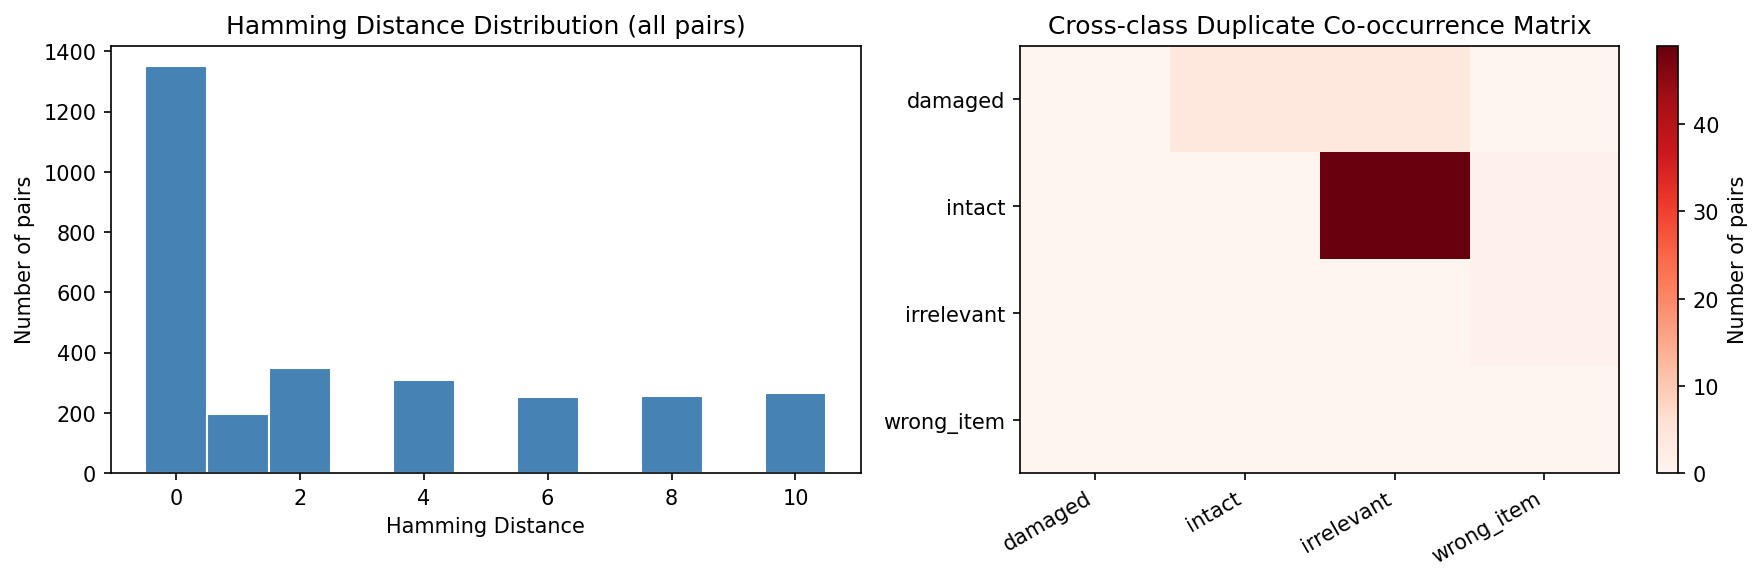
\includegraphics[width=\textwidth]{graphics/duplicate_analysis.png}
    \caption{Phân phối khoảng cách Hamming toàn bộ cặp trùng lặp (trái) và ma
        trận đồng xuất hiện trùng lặp liên nhãn (phải).}
    \label{fig:duplicate_analysis}
\end{figure}

Phân phối khoảng cách Hamming cho thấy khoảng 1.350 cặp có khoảng cách bằng 0
--- tức trùng chính xác ở cấp độ nội dung thị giác --- và tần suất giảm dần
khi khoảng cách tăng lên đến ngưỡng 10. Đáng chú ý, ma trận đồng xuất hiện
liên nhãn cho thấy cặp \texttt{intact}--\texttt{irrelevant} có tần suất cao
nhất (~35 cặp), tiếp theo là cặp \texttt{damaged}--\texttt{intact}. Trong số 90 cặp cross-class, có 46 cặp trùng chính xác (khoảng cách Hamming = 0) --- đây là các trường hợp cùng một ảnh xuất hiện dưới hai nhãn khác nhau, có khả năng cao là do lỗi gán nhãn hoặc ảnh bị mượn từ nhóm nhãn khác trong quá trình thu thập. Danh sách 46 cặp này đã được xuất ra tệp
